\documentclass[
	    a4paper, 				%Papierformat
	    bibliography=totocnumbered,		%Literaturverzeichnis im Inhaltsverzeichnis
	    listof=totocnumbered,		%Tabellen/Abbildungen im Inhaltszverzeichnis
	    11pt, 				%Schriftgröße
]{scrreprt}

%%%%%%%%%%%%%%%%%%%%%%%%%%%%%%%%%%%%%%%%%%%%%%%%%%%%%%%%%%%%%%%%%%%%%%%%%%%%%%%%%%%%%%%%%%%%%%
%% Packages

	\usepackage[english]{babel}  %Anpassung an englische Sprache von Formaten (z.B. Datum)
	\usepackage{csquotes}
	\usepackage{pdfpages} %anzeigen von PDFs
	\usepackage{fontspec} %Schriftarten für LuaLaTeX
	\usepackage{nomencl} %Abkürzungsverzeichnis makeindex Dissertation.nlo -s nomencl.ist -o Dissertation.nls
	\usepackage{etoolbox} %Abkürzungsverzeichnis im Inhaltsverzeichnis
	\usepackage{siunitx} %si units
	\usepackage[a4paper]{geometry} %Seitenlayout
	\usepackage{tabularx} %Tabellenpaket
	\usepackage{multirow} %Reihen in Tabellen zusammenfassen
	\usepackage[colorlinks,pdfpagelabels,pdfstartview = FitH, bookmarksopen = true, 
		    bookmarksnumbered = true, linkcolor = black, plainpages = false,
		    hypertexnames = false, citecolor = black] {hyperref} % pdf Verlinkung
	\usepackage{longtable} %lange Tabellen
	\usepackage{verbatim} %lange Kommentare
	\usepackage{caption} %verschiedene Caption befehle
	\usepackage{subcaption}
	\usepackage{textcomp} %Promille zeichen
	\usepackage{microtype} %verbessert die Zeilenbreite durch minimale Veränderungen der Buchstabenbreite
	
	%%%%%%%%%%%%%%%%%%%%%%%%%%%%%%%%%%%%%%%%%%%%%%%%%%%%%%%%%%%%%%%%%%%%%%%%%%%%%%%%%%%%%%%%%%%%%%
	%% Bib
	
	\usepackage[
		style=authoryear,
		backend=biber, %using biber as bbl generator
		block=par,
		natbib=true, %enables \citep
		giveninits=true, %shows initials instead of full names in bib
		uniquename=false, 
		dashed=false %Fully write authornames instead of --- when they appear multiple times
	]{biblatex}
	\addbibresource{library.bib}
	\ExecuteBibliographyOptions{
		isbn=false,
		doi=false,
		url=false,
		maxbibnames=1000,
		maxcitenames=2,
		uniquelist=false
	}
	
	\DeclareNameAlias{default}{last-first} 
	\renewcommand*{\finalnamedelim}{\multinamedelim} %removes "and" from last author
	\DeclareFieldFormat*{title}{#1} %removes formatting the title
	\DeclareFieldFormat*{journaltitle}{#1} %removes formatting the journal
	\DeclareFieldFormat{pages}{#1} %removes pp
	\DeclareFieldFormat*{volume}{\underline{#1}} %underline volume
	
	\defbibenvironment{bibliography} %add numeration
		{\enumerate
			{}
			{\setlength{\leftmargin}{\bibhang}%
				\setlength{\itemindent}{-\leftmargin}%
				\setlength{\itemsep}{\bibitemsep}%
				\setlength{\parsep}{\bibparsep}}}
		{\endenumerate}
		{\item}
	
	\renewbibmacro{in:}{} %removes in from journal
	\renewcommand{\labelnamepunct}{\addcolon} %colon after authors
	\AtEveryBibitem{\ifentrytype{article}{\clearfield{number}}{}} %remove issue number
	

%%%%%%%%%%%%%%%%%%%%%%%%%%%%%%%%%%%%%%%%%%%%%%%%%%%%%%%%%%%%%%%%%%%%%%%%%%%%%%%%%%%%%%%%%%%%%%
%% ZeilenAbstand

	\usepackage[onehalfspacing]{setspace} %Zeilenabstand

%%%%%%%%%%%%%%%%%%%%%%%%%%%%%%%%%%%%%%%%%%%%%%%%%%%%%%%%%%%%%%%%%%%%%%%%%%%%%%%%%%%%%%%%%%%%%%
%% Schriftart
	\setmainfont{Arial}
	\setsansfont{Arial}

%%%%%%%%%%%%%%%%%%%%%%%%%%%%%%%%%%%%%%%%%%%%%%%%%%%%%%%%%%%%%%%%%%%%%%%%%%%%%%%%%%%%%%%%%%%%%%
%% Seitenlayout

	\geometry{a4paper, left=30mm, right=25mm, top=25mm, bottom=25mm}
	\setlength{\headheight}{1.1\baselineskip}
	
%%%%%%%%%%%%%%%%%%%%%%%%%%%%%%%%%%%%%%%%%%%%%%%%%%%%%%%%%%%%%%%%%%%%%%%%%%%%%%%%%%%%%%%%%%%%%%
%% Abkürzungsverzeichnis

	\patchcmd{\thenomenclature}{\chapter*}{\chapter}{} {} %Abkürzungsverzeichnis nummeriert im Inhaltsverzeichnis   
	\let\abk\nomenclature	%Befehl umbenennen in abk 
	%\setlength{\nomlabelwidth}{0.3\hsize}         
	%\renewcommand{\nomlabel}[1]{#1 \dotfill}      %Füllt mit Punkten auf 
	\setlength{\nomitemsep}{-\parsep} 
	\makenomenclature               %Erzeugt Abkürzungsverzeichnis
	
%%%%%%%%%%%%%%%%%%%%%%%%%%%%%%%%%%%%%%%%%%%%%%%%%%%%%%%%%%%%%%%%%%%%%%%%%%%%%%%%%%%%%%%%%%%%%%
%% Kopfnoten und Seitenzahl

	\usepackage[headsepline,plainheadsepline]{scrpage2}
	\pagestyle{scrheadings}
	\ihead[\rightmark]{\rightmark} \chead[]{}
	\automark{chapter}
	\renewcommand{\chaptermark}[1]{\markright{\ #1}}

%%%%%%%%%%%%%%%%%%%%%%%%%%%%%%%%%%%%%%%%%%%%%%%%%%%%%%%%%%%%%%%%%%%%%%%%%%%%%%%%%%%%%%%%%%%%%%
%% Inhaltsverzeichnis Einstellungen

	\setcounter{tocdepth}{3} %Abschnittstiefe, die im Inhaltsverzeichnis dargestellt wird
	\setcounter{secnumdepth}{3} %Abschnittstiefe, die noch nummeriert wird

%%%%%%%%%%%%%%%%%%%%%%%%%%%%%%%%%%%%%%%%%%%%%%%%%%%%%%%%%%%%%%%%%%%%%%%%%%%%%%%%%%%%%%%%%%%%%%
%% Hauptdokument

\begin{document}


	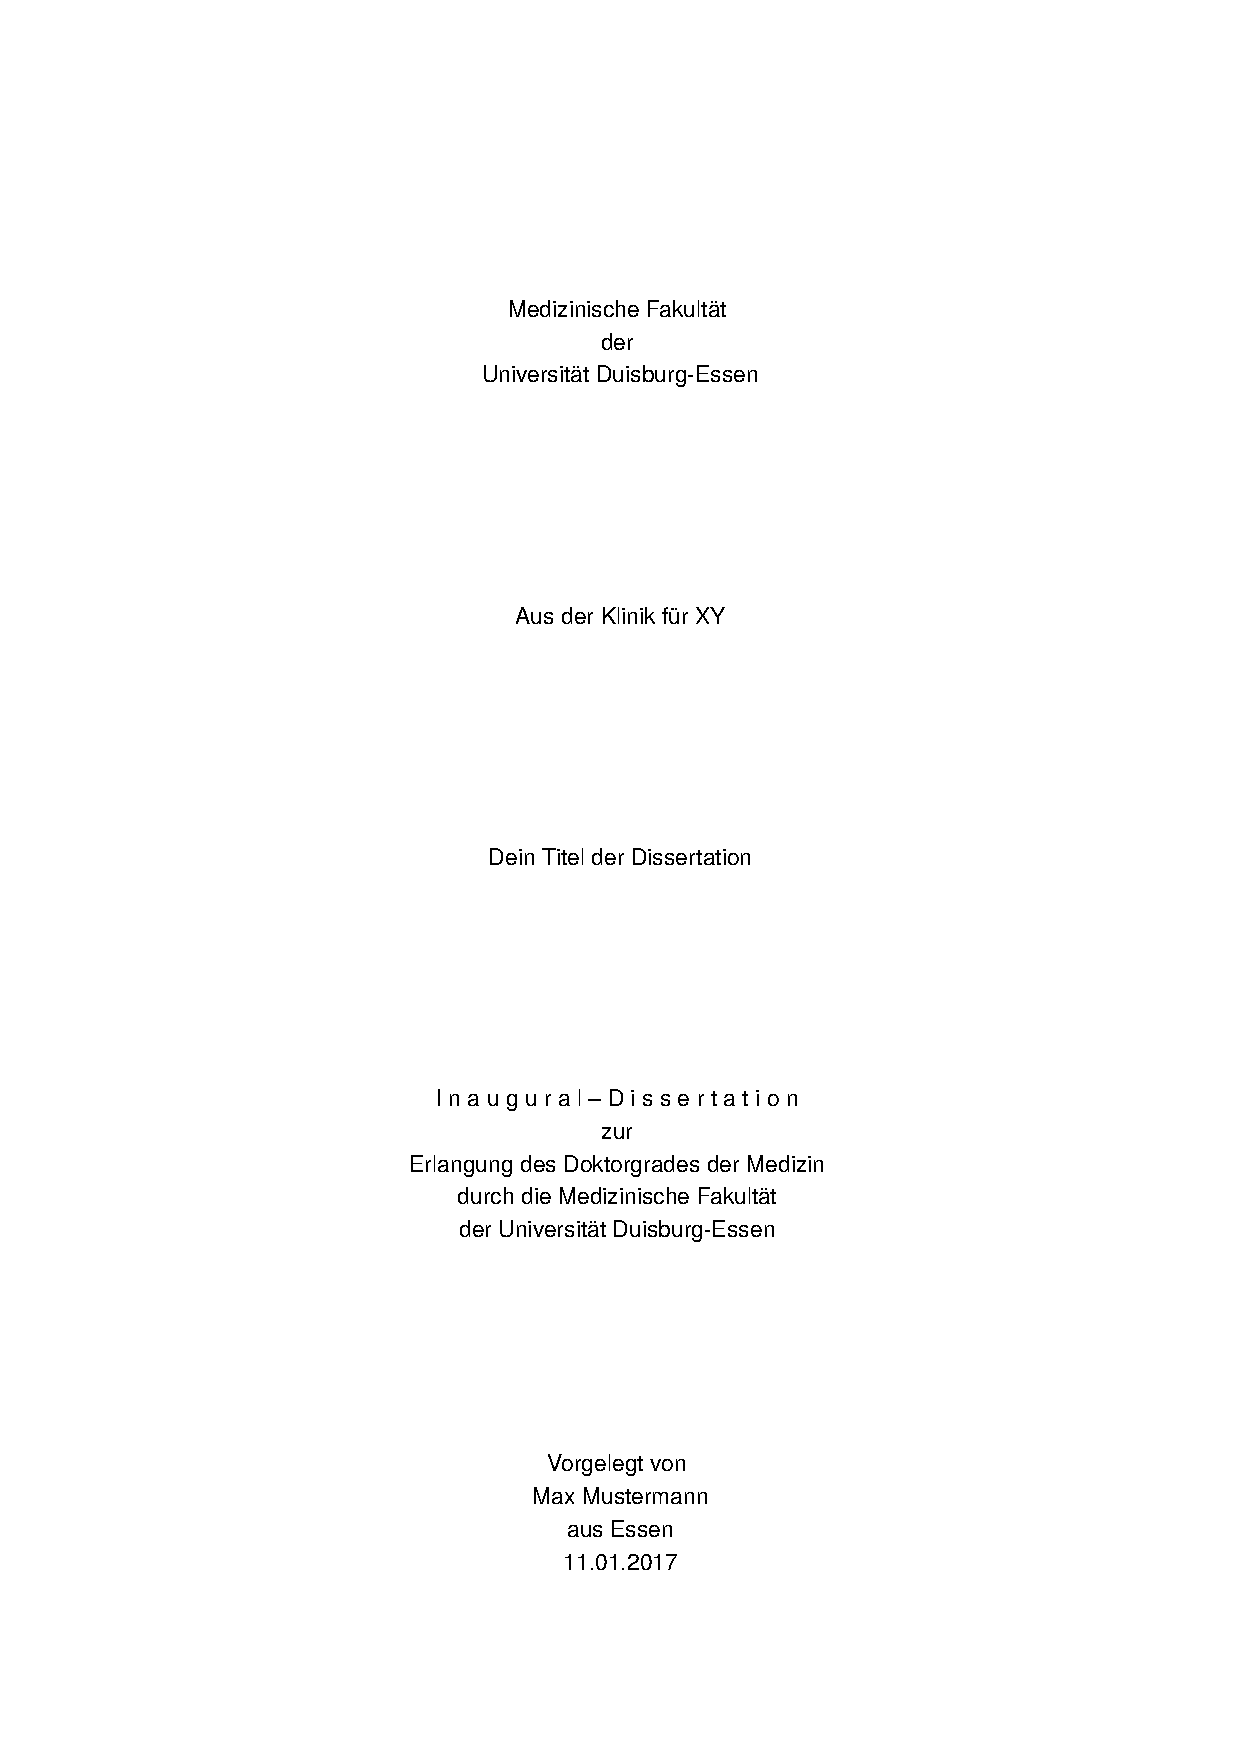
\includepdf{Titelseite.pdf}
	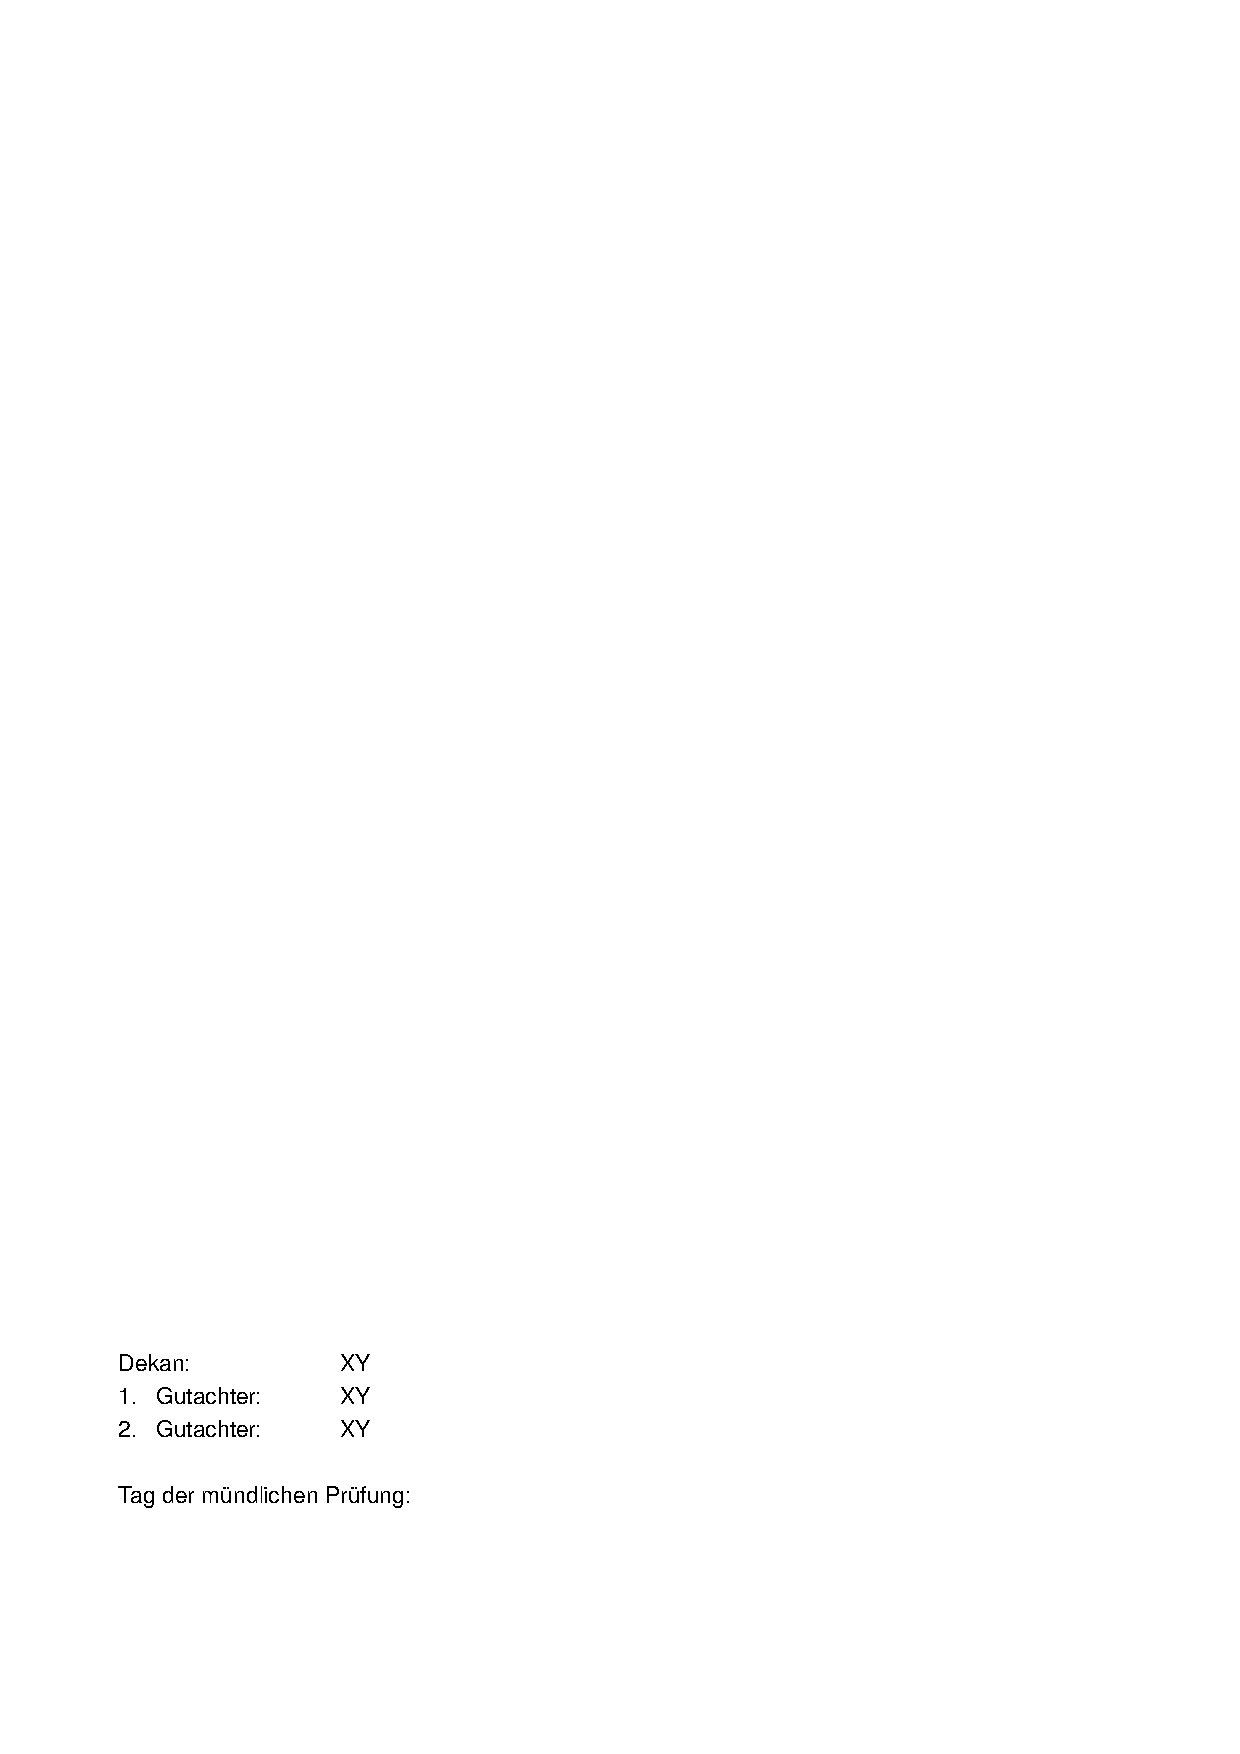
\includepdf{ZweiteSeite.pdf}
	
\includepdf{Publikationen.pdf}
	\tableofcontents

	
	\chapter{Introduction}
		Write your introduction here. Zitation \citep{Lesley2004}
		\par
		%Abkürzungsverzeichnis makeindex Dissertation.nlo -s nomencl.ist -o Dissertation.nls
		Abkürzung LPS (Lipopolysaccharide)\abk{LPS}{Lipopolysaccharide}

	\chapter{Materials and methods}
		\section{Materials}
			\subsection{Chemicals}
	  

				\begin{longtable}{||l|r||}
						Item&Manufacturer\\
					\hline\hline
						\multirow{2}{0.62\textwidth}{Antikörper}&
						\multirow{2}{0.30\textwidth}{Firma}\\&\\	
					\hline\hline
					\caption{Antibodies}
				\end{longtable}
				\begin{longtable}{||l|r||}
							Item&Manufacturer\\
						\hline\hline
							\multirow{2}{0.62\textwidth}{Primer}&
							\multirow{2}{0.30\textwidth}{Firma}\\&\\			
						\hline\hline	
						\caption{Primer}
					\end{longtable}
					\begin{longtable}{||l|r||}
							Item&Manufacturer\\
						\hline\hline
							\multirow{2}{0.62\textwidth}{Milk powder Blotting grade}&
							\multirow{2}{0.30\textwidth}{Carl Roth GmbH + Co. KG, 76185 Karlsruhe, Germany}\\&\\
						\hline\hline
						\caption{Solid substances}
					\end{longtable}
					\begin{longtable}{||l|r||}
							Item&Manufacturer\\
						\hline\hline
							\multirow{3}{0.62\textwidth}{NaCl 0.9\%}&
							\multirow{3}{0.30\textwidth}{B. Braun Melsungen AG, 34209 Melsungen, Germany}\\&\\&\\
						\hline\hline
						\caption{Fluids}
					\end{longtable}
					\begin{longtable}{||l|r||}
							Item&Manufacturer\\
						\hline\hline
							\multirow{2}{0.62\textwidth}{Amersham ECL Plus}&
							\multirow{2}{0.30\textwidth}{GE Healthcare, 42655 Solingen, Germany}\\&\\
						\hline\hline
					\caption{Kits}
				\end{longtable}

				
			\subsection{Buffers and solutions}
				\subsubsection{General solutions}
					\begin{itemize}
						\item Phosphat buffered saline (PBS)\abk{PBS}{Phosphat buffered saline}, pH 7.4
						\begin{itemize}
							\item 137 mM NaCl
							\item 2.7 mM KCl
							\item 12 mM phosphate
							\item Titrate to pH 7.4 with HCl
						\end{itemize}
					\end{itemize}
			\subsection{Equipment}
				\begin{longtable}{||l|r||}
						Device&Manufacturer\\
					\hline\hline
						\multirow{3}{0.62\textwidth}{NanoDrop 1000 Spectrophotometer}&
						\multirow{3}{0.30\textwidth}{NanoDrop products, Wilmington, DE 19810, USA}\\&\\&\\							
					\hline\hline				
					\caption{Equipment}
				\end{longtable}
				
			\subsection{Instruments}
			
				\begin{longtable}{||l|r||}
						Instrument&Manufacturer\\
					\hline\hline
						\multirow{3}{0.62\textwidth}{100 µl Hamilton-Pipette (710n 22s/51/2)}&
						\multirow{3}{0.30\textwidth}{Hamilton Robotics, CH-7402 Bonaduz, GR, Switzerland}\\&\\&\\
					\hline\hline			
					\caption{Instruments}
				\end{longtable}
	  
			\subsection{Disposables}
			
				\begin{longtable}{||l|r||}
					Instrument&Manufacturer\\
					\hline\hline
						\multirow{2}{0.62\textwidth}{1.5 ml/2.0 ml reaction tubes}&
						\multirow{2}{0.30\textwidth}{Eppendorf AG, 22339 Hamburg, Germany}\\&\\										
					\hline\hline
					\caption{Disposables}
				\end{longtable}
		
		\section{Methods}		

	\chapter{Results}
		Write your results here
		Figure
		

		\begin{figure}
			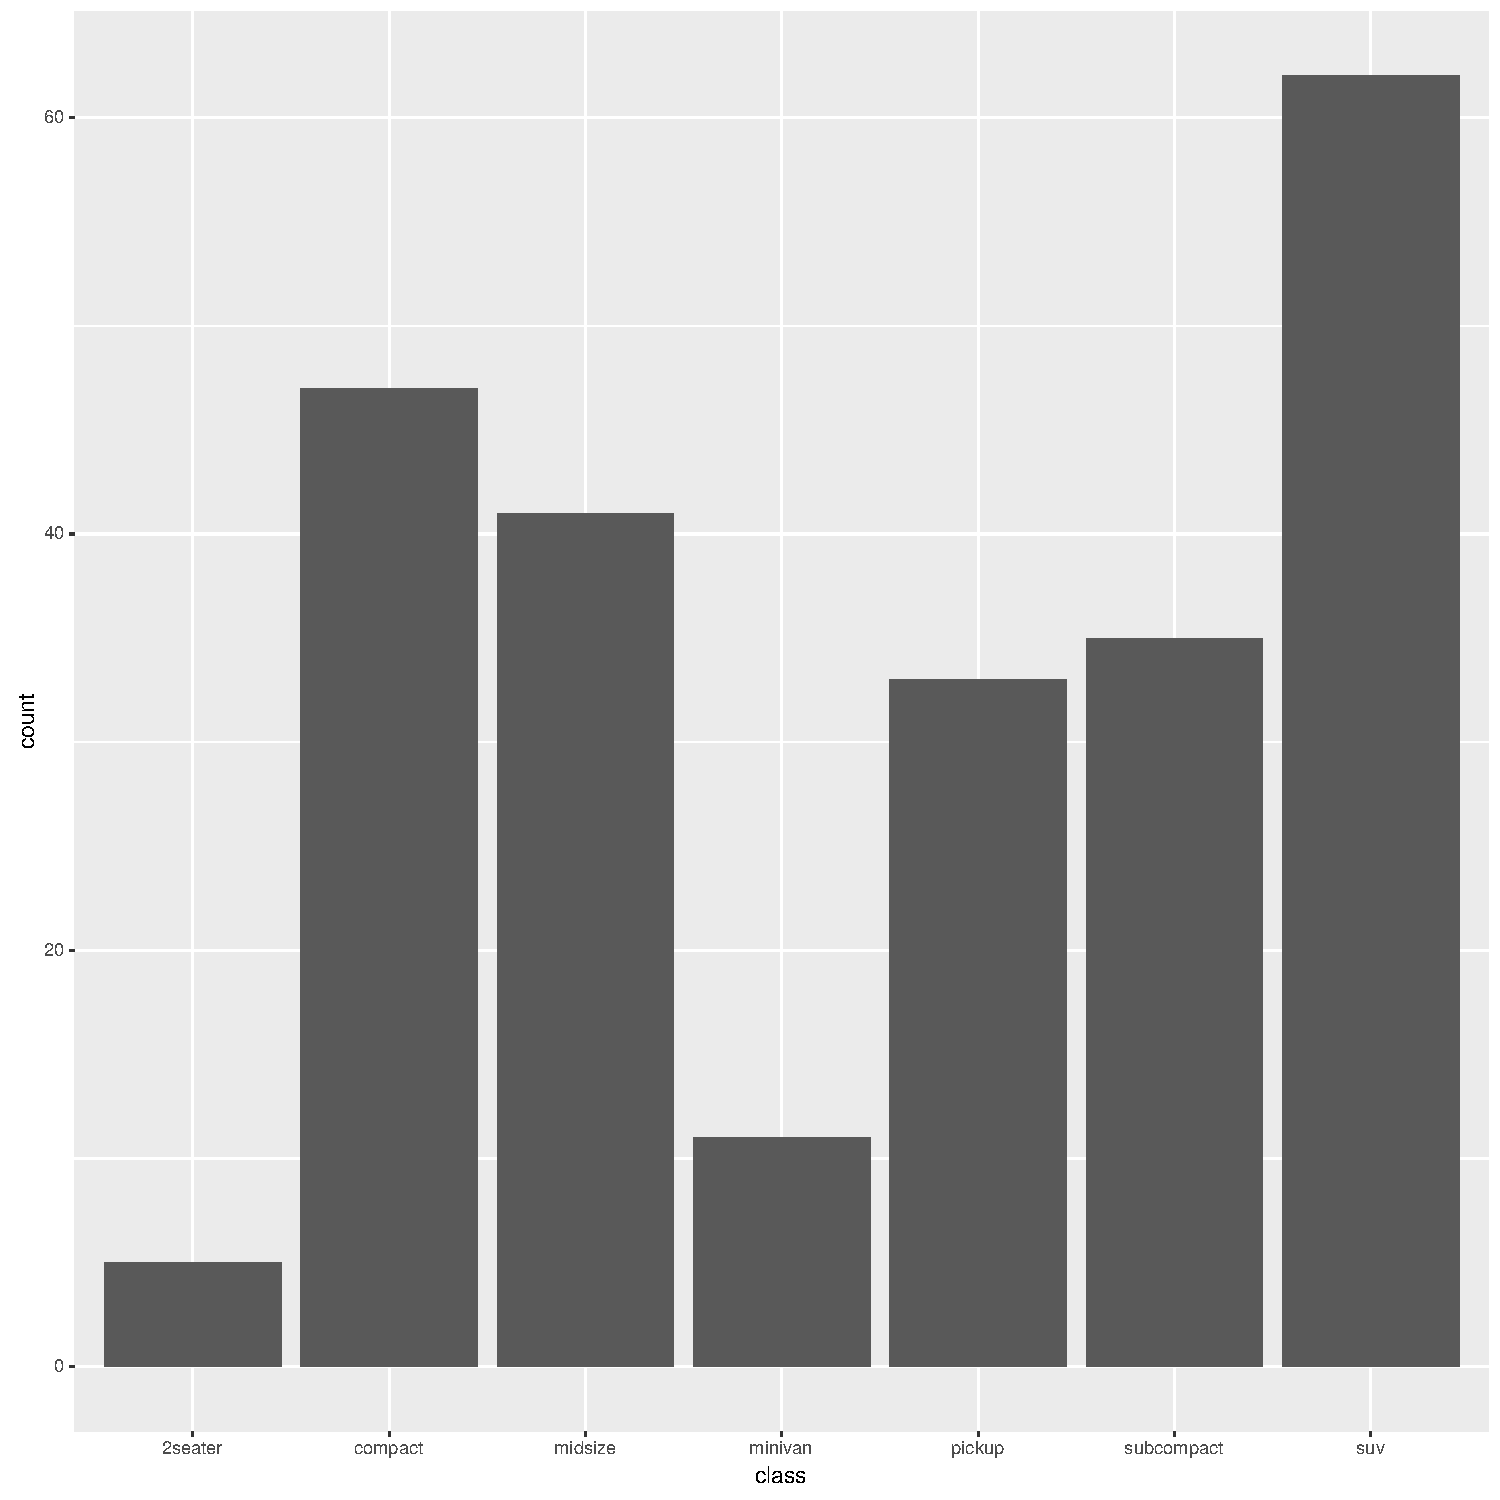
\includegraphics[width=\textwidth]{images/barplot.pdf}
			\caption{\textbf{Fantastic image} 
				\newline 
				Explain what the image means.
				\newline
				\textit{Method:} Whatever, 
				\textit{samples:} Tissue/n = 1-5, 
				\textit{treatment:} Whatever, 
				\textit{graphics:} bar plots,
				\textit{statistics:} pairwise t-test
			}
			\label{barplot}
		\end{figure}

	\chapter{Discussion}
		Write your discussion here
				
	\chapter{Conclusion}
		Write your conclusion here
		
	\chapter{Abstract}
		\textit{Introduction}: 
		\par 
		\textit{Methods}: 
		\par
		\textit{Results}: 
		\par
		\textit{Conclusion}: 


%%%%%%%%%%%%%%%%%%%%%%%%%%%%%%%%%%%%%%%%%%%%%%%%%%%%%%%%%%%%%%%%%%%%%%%%%%%%%%%%%%%%%%%%%%%%%%%%%%%%%%%%%%%%%%%%%%%%%%%%%%%%%%%%%
%% Anhang

	\appendix
	\printbibliography
	\listoftables
	\listoffigures
	\printnomenclature
	\chapter{Acknowledgement}  
	Write your acknowledgement here
	
	
\includepdf[pages={1}]{Lebenslauf.pdf}
	%include papers here
	%\includepdf[pages={1-7}]{paper}


\end{document}          